\chapter{Results} \label{chap:results}

The experiments previously outlined produced a series of CSV files, which were aggregated and evaluated into one list of findings\footnote{The full simulation output is accessible at this URL: \url{https://stack.gandreadis.com/s/nb5QbGWhPIRpM64}}. In general, this result data exhibits a higher throughput for both pedestrians and cars in the larger crosswalk map compared to the smaller crosswalk map. Figure \ref{fig:plot-pedestrian-throughput} and \ref{fig:plot-car-throughput} plot pedestrian and car throughput (respectively) against varying spawn delays. These varying delays indicate different levels of load on the layout, where higher delay translates to lower load. Each point on the charts represents the average of ten repetitions in that configuration, to eliminate non-deterministic factors.

\begin{figure}[h]
    \centering
    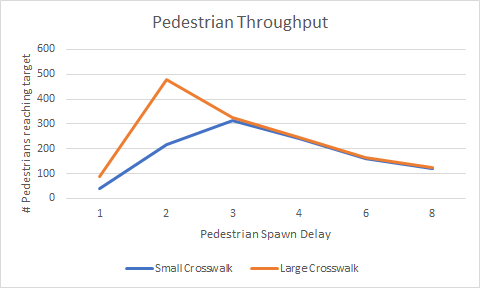
\includegraphics[width=4.1in]{images/plot-pedestrian-throughput.png}
    \caption{Plot of pedestrian throughput against pedestrian spawn delay, for both map layouts (car spawn delay is fixed at 5).}
    \label{fig:plot-pedestrian-throughput}
\end{figure}

\begin{figure}[h]
    \centering
    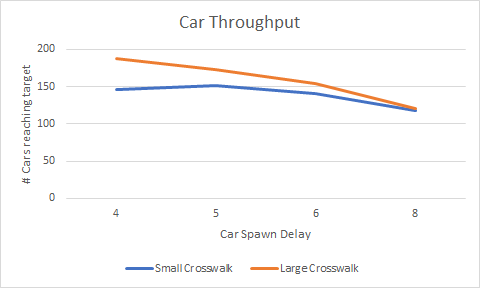
\includegraphics[width=4.1in]{images/plot-car-throughput.png}
    \caption{Plot of car throughput against car spawn delay, for both map layouts (pedestrian spawn delay is fixed at 5).}
    \label{fig:plot-car-throughput}
\end{figure}

Figure \ref{fig:plot-pedestrian-throughput} shows pedestrian throughput over pedestrian spawn delays. At low spawn delay (1-2), the simulation quickly becomes crowded, and the larger crosswalk has significantly higher throughput. At higher delays (3+), congestion ceases to be an issue and this difference becomes negligible. Figure \ref{fig:plot-car-throughput}, on the other hand, shows a more consistent decline of car throughput over car spawn delay. The car throughput of the large crosswalk layout remains consistently greater than the car throughput of the small crosswalk. However, this difference decreases at longer car spawn delays, and the margin of performance between the two maps also becomes negligible.

Both of the central results shown in Figure \ref{fig:plot-pedestrian-throughput} and \ref{fig:plot-car-throughput} look at the average throughputs over iterations. To make certain that the average values were representative of their series, the variance of each series was also calculated. This variance decreased with decreasing traffic density, but stayed low throughout. Figures \ref{fig:plot-pedestrian-variance} and \ref{fig:plot-car-variance} show this effect for pedestrians and cars, respectively.

\begin{figure}[h]
    \centering
    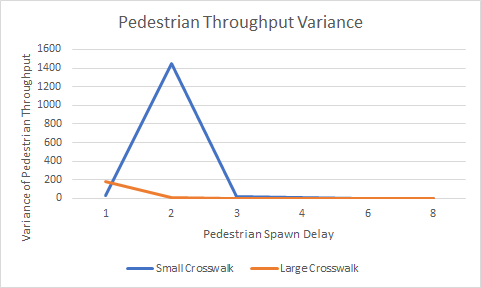
\includegraphics[width=4.1in]{images/plot-pedestrian-variance.png}
    \caption{Plot of pedestrian throughput variance against pedestrian spawn delay, for both map layouts (car spawn delay is fixed at 5).}
    \label{fig:plot-pedestrian-variance}
\end{figure}

\begin{figure}[h]
    \centering
    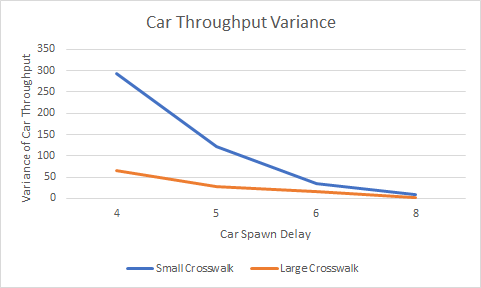
\includegraphics[width=4.1in]{images/plot-car-variance.png}
    \caption{Plot of car throughput variance against car spawn delay, for both map layouts (pedestrian spawn delay is fixed at 5).}
    \label{fig:plot-car-variance}
\end{figure}

We also recorded the number of failed spawn attempts for each run. However, as this data is complementary to the throughput data, the one can be derived from the other (given the total number of agents of that type spawned). It thus provides little additional information, and will not be discussed further in this report.